%!TEX program = xelatex
% 完整编译: xelatex -> biber/bibtex -> xelatex -> xelatex
\documentclass[lang=cn,11pt,a4paper]{elegantpaper}

\title{python中的数据处理2}
\author{杨晨 \\学号2021212171}
\institute{北京邮电大学 计算机学院}

% \version{0.10}
\date{\zhtoday}

% 本文档命令
\usepackage{array}
\usepackage{xcolor}
\usepackage{float}
\newcommand{\ccr}[1]{\makecell{{\color{#1}\rule{1cm}{1cm}}}}

% 设置全局代码样式
\lstset{
  language=Python, % 设置语言为Python
  keywordstyle=\color{blue}, % 设置关键字颜色为蓝色
  commentstyle=\color{green!60!black}, % 设置注释颜色为绿色
  stringstyle=\color{orange}, % 设置字符串颜色为橙色
  showstringspaces=false, % 不显示字符串中的空格
  frame=single, % 添加边框
  breaklines=true, % 自动断行
  numberstyle=\tiny\color{gray}, % 设置行号样式为小号灰色
  captionpos=b % 设置标题位置为底部
}
 
\lstdefinelanguage{text}{
    showstringspaces=false,
    breaklines=true,
    breakatwhitespace=true,
    tabsize=4
}

\begin{document}



\maketitle
% \tableofcontents

\section{概述}

\subsection{实验内容}

处理北京空气质量数据。

\begin{enumerate}
    \item 对PM指数进行异常值的处理:假设PM指数最高为500,将PM\_Dongsi、PM\_Dongsihuan、PM\_Nongzhanguan三列中超过500的数据,修改为500。 
    \item 对PRES和TEMP数据进行最大最小归一化和标准化归一化,并使用散点图进行展示。
    \item 针对北京每天的PM平均值(对多个测试站点和多个时间的值求平均),统计不同颜色代表的指数等级(指数等级见课件第23页)各有多少天。
\end{enumerate}

\subsection{开发环境}

\begin{itemize}
    \item Windows10
    \item PyCharm 2023.2.4 (Professional Edition)
\end{itemize}

\section{实验过程}

\subsection{对PM异常值的处理}
数据预处理的第一步是将数据集加载到 Pandas 的 DataFrame 中。检查三个地点(PM\_Dongsi、PM\_Dongsihuan、PM\_Nongzhanguan)的PM2.5浓度值是否超过500,如果超过则用500代替。
\begin{lstlisting}[language=python]
df = pd.read_csv('BeijingPM20100101_20151231.csv', encoding='utf-8')

# 将PM_Dongsi、PM_Dongsihuan、PM_Nongzhanguan三列中超过500的数据,修改为500。
df.loc[df['PM_Dongsi'] > 500, 'PM_Dongsi'] = 500
df.loc[df['PM_Dongsihuan'] > 500, 'PM_Dongsihuan'] = 500
df.loc[df['PM_Nongzhanguan'] > 500, 'PM_Nongzhanguan'] = 500
\end{lstlisting}

然后将处理过的数据保存到 CSV 文件中。

\begin{lstlisting}[language=python]
# 保存处理后的数据
df.to_csv('data.csv', index=False)
\end{lstlisting}

\subsection{归一化}
接下来,使用最小最大归一化和标准化归一化方法对气压(PRES)和温度(TEMP)变量进行归一化处理。最小-最大归一化将数值映射到 0 和 1 之间的范围,而标准化归一化则将数据转换为平均值为 0,标准偏差为 1。
\begin{lstlisting}[language=python]
# 对PRES和TEMP数据进行最大最小归一化和标准化归一化
x_reshape = df['PRES'].values.reshape(-1, 1)
y_reshape = df['TEMP'].values.reshape(-1, 1)

# 最大最小归一化
min_max_scaler = MinMaxScaler()
normalized_pres = min_max_scaler.fit_transform(x_reshape)
normalized_temp = min_max_scaler.fit_transform(y_reshape)

# 标准化归一化
standard_scaler = StandardScaler()
standardized_pres = standard_scaler.fit_transform(x_reshape)
standardized_temp = standard_scaler.fit_transform(y_reshape)
\end{lstlisting}

为了直观显示变量之间的关系,绘制了散点图。生成了三个散点图,分别代表不同的归一化方法:原始、最大最小归一化和标准化归一化。每个散点图的 x 轴代表气压(PRES),y 轴代表温度(TEMP)。通过散点图,可以分析不同归一化技术下气压和温度之间的相关性。
\begin{lstlisting}[language=python]
# 绘制散点图
fig, axes = plt.subplots(1, 3, figsize=(15, 8))
axes[0].scatter(df['PRES'], df['TEMP'], marker='o')
axes[1].scatter(normalized_pres, normalized_temp, marker='o')
axes[2].scatter(standardized_pres, standardized_temp, marker='o')
axes[0].set_xlabel('PRES')
axes[0].set_ylabel('TEMP')
axes[0].set_title('Original')
axes[1].set_xlabel('normalized PRES')
axes[1].set_ylabel('normalized TEMP')
axes[1].set_title('Normalized')
axes[2].set_xlabel('standardized PRES')
axes[2].set_ylabel('standardized TEMP')
axes[2].set_title('Standardized')
fig.tight_layout()
plt.savefig('scatter.png')
plt.show()
\end{lstlisting}

\begin{figure}[H]
    \centering
    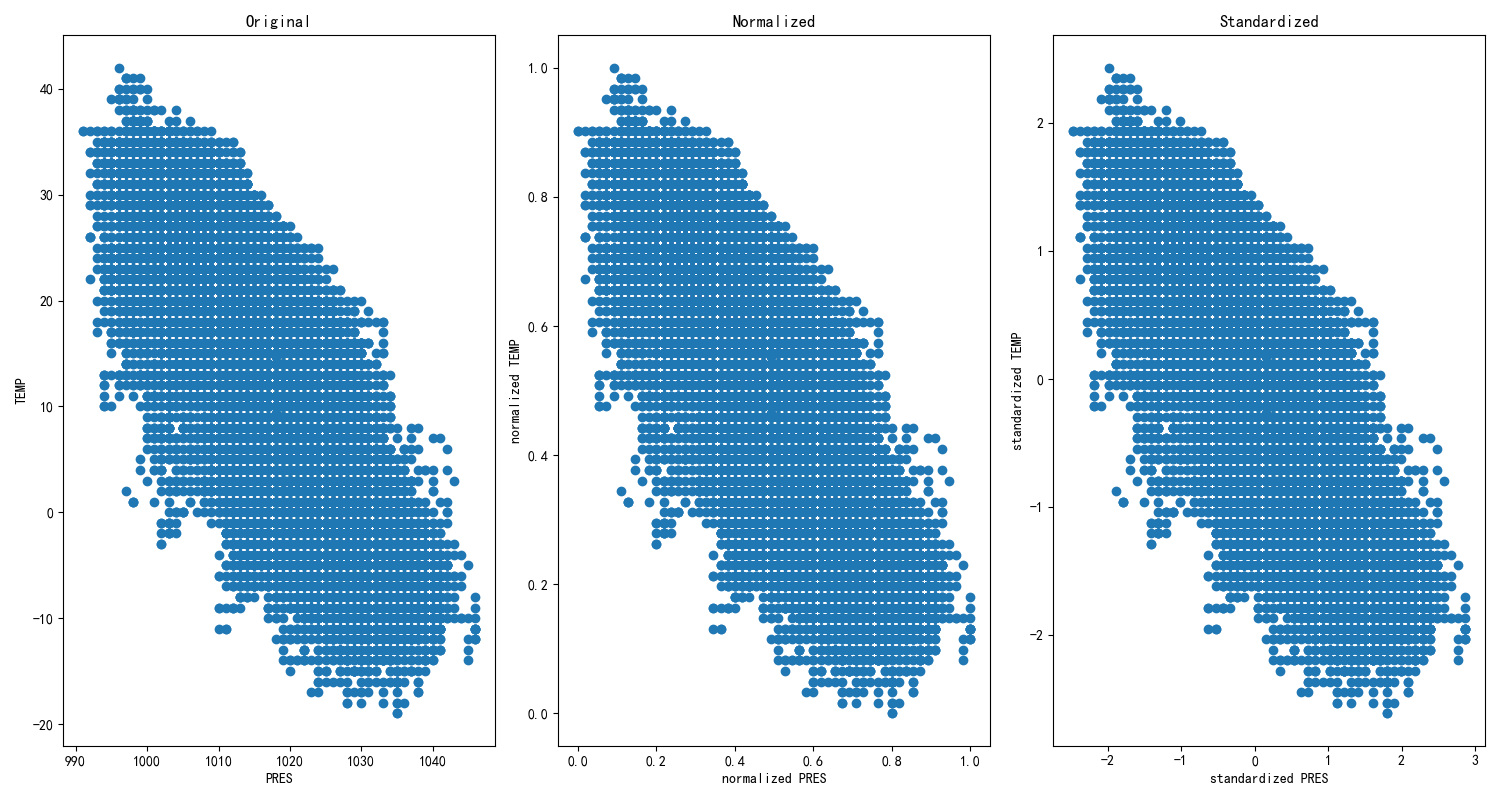
\includegraphics[width=0.9\textwidth]{image/scatter.png}
    \caption{散点图}
\end{figure}

\subsection{统计污染情况}
通过取三个地点 PM2.5 浓度的平均值,创建了一个新列 PM\_avg。然后按年、月、日对数据集进行分组,并计算出每组的 PM\_avg 的平均值。处理后的数据被保存,只保留年、月、日和 PM\_avg 列。
\begin{lstlisting}[language=python]
# 新建一列,将PM_Dongsi、PM_Dongsihuan、PM_Nongzhanguan三列的数据进行平均,赋值给新建的列PM_avg
df['PM_avg'] = df[['PM_Dongsi', 'PM_Dongsihuan', 'PM_Nongzhanguan']].mean(axis=1)
# 按照year、month、day进行分组,求PM_avg的平均值
df = df.groupby(['year', 'month', 'day'])['PM_avg'].mean()
# 保存处理后的数据,只保留year、month、day和PM_avg四列
df.to_csv('data1.csv', index=True, header=True)
\end{lstlisting}

\begin{figure}[H]
    \centering
    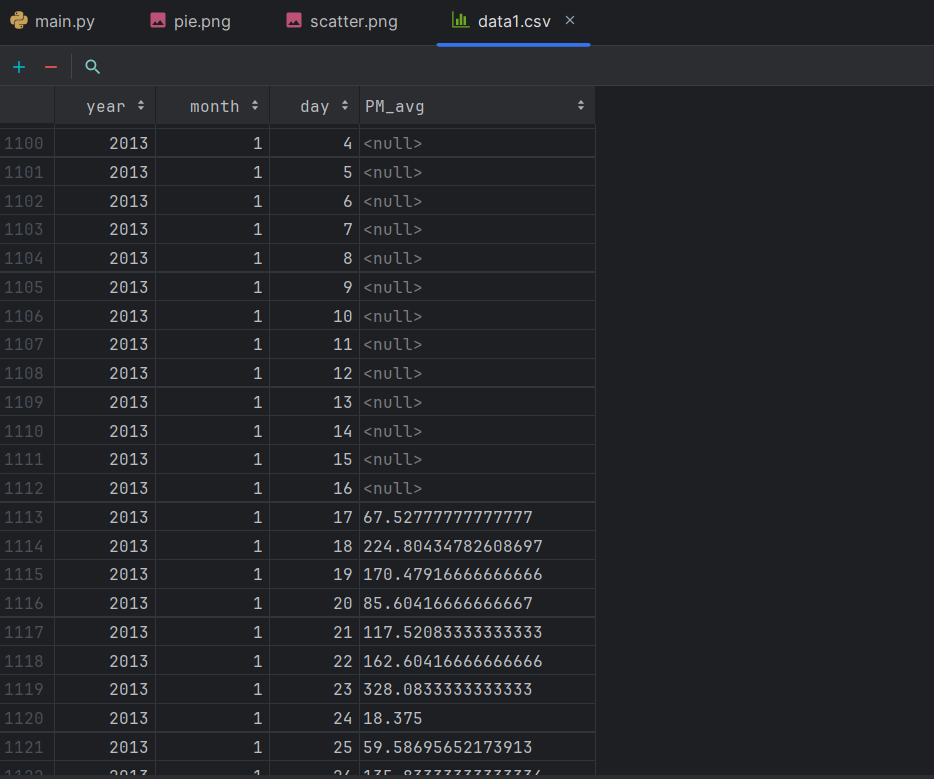
\includegraphics[width=0.9\textwidth]{image/data1.png}
    \caption{data1.csv}
\end{figure}

为了对污染程度进行分类,PM平均值被分为不同的部分: 0-50、51-100、101-150、151-200、201-300 和 301-500。这些区段分别被标记为 "优"、"良"、"轻度污染"、"中度污染"、"重度污染"和 "严重污染"。计算了属于每个污染等级类别的天数,并用饼状图将其直观显示出来。

\begin{lstlisting}[language=python]
sections = [0, 50, 100, 150, 200, 300, 501]
sections_color = ['green', 'yellow', 'orange', 'red', 'purple', 'maroon']
sections_name = ['优', '良', '轻度污染', '中度污染', '重度污染', '严重污染']
result = pd.cut(df, sections, labels=sections_name)
# 统计各个污染程度的天数
print(pd.value_counts(result))
# 绘制饼图
plt.figure(figsize=(6, 6))
plt.pie(pd.value_counts(result), labels=sections_name, colors=sections_color, autopct='%1.1f%%')
plt.title('Beijing PM2.5')
plt.savefig('pie.png')
plt.show()
\end{lstlisting}

统计结果如下:
\begin{lstlisting}[language=text]
优       375
良       337
轻度污染    191
中度污染     77
重度污染     74
严重污染     25
Name: PM_avg, dtype: int64
\end{lstlisting}

\begin{figure}[H]
    \centering
    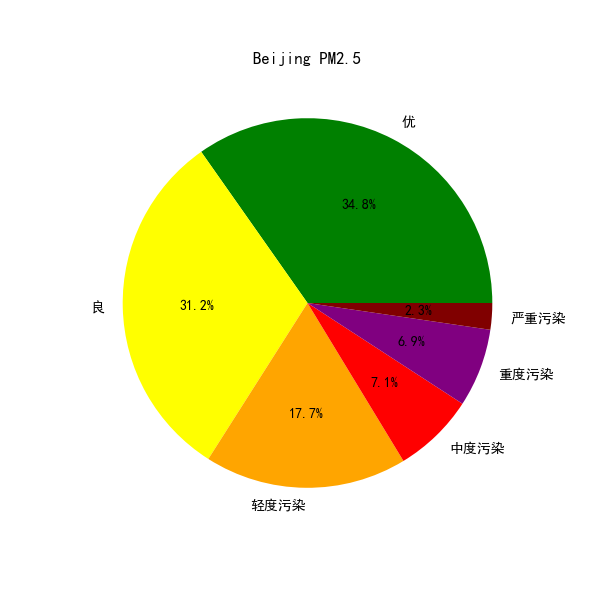
\includegraphics[width=0.9\textwidth]{image/pie.png}
    \caption{饼图}
\end{figure}


\section{附录:完整代码}

\begin{lstlisting}
import pandas as pd
from sklearn.preprocessing import MinMaxScaler, StandardScaler
import matplotlib.pyplot as plt
import matplotlib

# 设置中文显示
matplotlib.rc("font", family="SimHei", weight="bold")
plt.rcParams["axes.unicode_minus"] = False

df = pd.read_csv('BeijingPM20100101_20151231.csv', encoding='utf-8')

# 将PM_Dongsi、PM_Dongsihuan、PM_Nongzhanguan三列中超过500的数据,修改为500。
df.loc[df['PM_Dongsi'] > 500, 'PM_Dongsi'] = 500
df.loc[df['PM_Dongsihuan'] > 500, 'PM_Dongsihuan'] = 500
df.loc[df['PM_Nongzhanguan'] > 500, 'PM_Nongzhanguan'] = 500

# 保存处理后的数据
df.to_csv('data.csv', index=False)

# 对PRES和TEMP数据进行最大最小归一化和标准化归一化
x_reshape = df['PRES'].values.reshape(-1, 1)
y_reshape = df['TEMP'].values.reshape(-1, 1)

# 最大最小归一化
min_max_scaler = MinMaxScaler()
normalized_pres = min_max_scaler.fit_transform(x_reshape)
normalized_temp = min_max_scaler.fit_transform(y_reshape)

# 标准化归一化
standard_scaler = StandardScaler()
standardized_pres = standard_scaler.fit_transform(x_reshape)
standardized_temp = standard_scaler.fit_transform(y_reshape)

# 绘制散点图
fig, axes = plt.subplots(1, 3, figsize=(15, 8))
axes[0].scatter(df['PRES'], df['TEMP'], marker='o')
axes[1].scatter(normalized_pres, normalized_temp, marker='o')
axes[2].scatter(standardized_pres, standardized_temp, marker='o')
axes[0].set_xlabel('PRES')
axes[0].set_ylabel('TEMP')
axes[0].set_title('Original')
axes[1].set_xlabel('normalized PRES')
axes[1].set_ylabel('normalized TEMP')
axes[1].set_title('Normalized')
axes[2].set_xlabel('standardized PRES')
axes[2].set_ylabel('standardized TEMP')
axes[2].set_title('Standardized')
fig.tight_layout()
plt.savefig('scatter.png')
plt.show()

# 新建一列,将PM_Dongsi、PM_Dongsihuan、PM_Nongzhanguan三列的数据进行平均,赋值给新建的列PM_avg
df['PM_avg'] = df[['PM_Dongsi', 'PM_Dongsihuan', 'PM_Nongzhanguan']].mean(axis=1)
# 按照year、month、day进行分组,求PM_avg的平均值
df = df.groupby(['year', 'month', 'day'])['PM_avg'].mean()
# 保存处理后的数据,只保留year、month、day和PM_avg四列
df.to_csv('data1.csv', index=True, header=True)

# 污染程度划分
sections = [0, 50, 100, 150, 200, 300, 501]
sections_color = ['green', 'yellow', 'orange', 'red', 'purple', 'maroon']
sections_name = ['优', '良', '轻度污染', '中度污染', '重度污染', '严重污染']
result = pd.cut(df, sections, labels=sections_name)
# 统计各个污染程度的天数
print(pd.value_counts(result))
# 绘制饼图
plt.figure(figsize=(6, 6))
plt.pie(pd.value_counts(result), labels=sections_name, colors=sections_color, autopct='%1.1f%%')
plt.title('Beijing PM2.5')
plt.savefig('pie.png')
plt.show()
\end{lstlisting}

% \subsection{全局选项}
% 此模板定义了一个语言选项 \lstinline{lang},可以选择英文模式 \lstinline{lang=en}(默认)或者中文模式 \lstinline{lang=cn}。当选择中文模式时,图表的标题引导词以及参考文献,定理引导词等信息会变成中文。你可以通过下面两种方式来选择语言模式:
% \begin{lstlisting}
% \documentclass[lang=cn]{elegantpaper} % or
% \documentclass{cn}{elegantpaper} 
% \end{lstlisting}

% \textbf{注意:} 英文模式下,由于没有添加中文宏包,无法输入中文。如果需要输入中文,可以通过在导言区引入中文宏包 \lstinline{ctex} 或者加入 \lstinline{xeCJK} 宏包后自行设置字体。 
% \begin{lstlisting}
% \usepackage[UTF8,scheme=plain]{ctex}
% \end{lstlisting}

% \subsection{数学字体选项}

% 本模板定义了一个数学字体选项(\lstinline{math}),可选项有三个:
% \begin{enumerate}
%   \item \lstinline{math=cm}(默认),使用 \LaTeX{} 默认数学字体(推荐,无需声明);
%   \item \lstinline{math=newtx},使用 \lstinline{newtxmath} 设置数学字体(潜在问题比较多)。
%   \item \lstinline{math=mtpro2},使用 \lstinline{mtpro2} 宏包设置数学字体,要求用户已经成功安装此宏包。
% \end{enumerate}

% \subsection{中文字体选项}

% 模板提供中文字体选项 \lstinline{chinesefont},可选项有
% \begin{enumerate}
%   \item \lstinline{ctexfont}:默认选项,使用 \lstinline{ctex} 宏包根据系统自行选择字体,可能存在字体缺失的问题,更多内容参考 \lstinline{ctex} 宏包\href{https://ctan.org/pkg/ctex}{官方文档}\footnote{可以使用命令提示符,输入 \lstinline{texdoc ctex} 调出本地 \lstinline{ctex} 宏包文档}。
%   \item \lstinline{founder}:方正字体选项(\textbf{需要安装方正字体}),后台调用 \lstinline{ctex} 宏包并且使用 \lstinline{fontset=none} 选项,然后设置字体为方正四款免费字体,方正字体下载注意事项见后文,用户只需要安装方正字体即可使用该选项。
%   \item \lstinline{nofont}:后台会调用 \lstinline{ctex} 宏包并且使用 \lstinline{fontset=none} 选项,不设定中文字体,用户可以自行设置中文字体,具体见后文。
% \end{enumerate}

% \subsubsection{方正字体选项}
% 由于使用 \lstinline{ctex} 宏包默认调用系统已有的字体,部分系统字体缺失严重,因此,用户希望能够使用其它字体,我们推荐使用方正字体。方正的{\songti 方正书宋}、{\heiti 方正黑体}、{\kaishu 方正楷体}、{\fangsong 方正仿宋}四款字体均可免费试用,且可用于商业用途。用户可以自行从\href{http://www.foundertype.com/}{方正字体官网}下载此四款字体,在下载的时候请\textbf{务必}注意选择 GBK 字符集,也可以使用 \href{https://www.latexstudio.net/}{\LaTeX{} 工作室}提供的\href{https://pan.baidu.com/s/1BgbQM7LoinY7m8yeP25Y7Q}{方正字体,提取码为:njy9} 进行安装。安装时,{\kaishu Win 10 用户请右键选择为全部用户安装,否则会找不到字体。}

% \begin{figure}[!htb]
% \centering
% 
\includegraphics[width=0.9\textwidth]{founder.png}
% \end{figure}

% \subsubsection{其他中文字体}
% 如果你想完全自定义字体\footnote{这里仍然以方正字体为例。},你可以选择 \lstinline{chinesefont=nofont},然后在导言区设置即可,可以参考下方代码:
% \begin{lstlisting}
% \setCJKmainfont[BoldFont={FZHei-B01},ItalicFont={FZKai-Z03}]{FZShuSong-Z01}
% \setCJKsansfont[BoldFont={FZHei-B01}]{FZKai-Z03}
% \setCJKmonofont[BoldFont={FZHei-B01}]{FZFangSong-Z02}
% \setCJKfamilyfont{zhsong}{FZShuSong-Z01}
% \setCJKfamilyfont{zhhei}{FZHei-B01}
% \setCJKfamilyfont{zhkai}[BoldFont={FZHei-B01}]{FZKai-Z03}
% \setCJKfamilyfont{zhfs}[BoldFont={FZHei-B01}]{FZFangSong-Z02}
% \newcommand*{\songti}{\CJKfamily{zhsong}}
% \newcommand*{\heiti}{\CJKfamily{zhhei}}
% \newcommand*{\kaishu}{\CJKfamily{zhkai}}
% \newcommand*{\fangsong}{\CJKfamily{zhfs}}
% \end{lstlisting}



% \subsection{自定义命令}
% 此模板并没有修改任何默认的 \LaTeX{} 命令或者环境\footnote{目的是保证代码的可复用性,请用户关注内容,不要太在意格式,这才是本工作论文模板的意义。}。另外,我自定义了 4 个命令:
% \begin{enumerate}
%   \item \lstinline{\email}:创建邮箱地址的链接,比如 \email{ddswhu@outlook.com};
%   \item \lstinline{\figref}:用法和 \lstinline{\ref} 类似,但是会在插图的标题前添加 <\textbf{图 n}> ;
%   \item \lstinline{\tabref}:用法和 \lstinline{\ref} 类似,但是会在表格的标题前添加 <\textbf{表 n}>;
%   \item \lstinline{\keywords}:为摘要环境添加关键词。
% \end{enumerate}

% \subsection{参考文献}

% 文献部分,本模板调用了 biblatex 宏包,并提供了 biber(默认) 和 bibtex 两个后端选项,可以使用 \lstinline{bibend} 进行修改:

% \begin{lstlisting}
%   \documentclass[bibtex]{elegantpaper}
%   \documentclass[bibend=bibtex]{elegantpaper}
% \end{lstlisting}

% 关于文献条目(bib item),你可以在谷歌学术,Mendeley,Endnote 中取,然后把它们添加到 \lstinline{reference.bib} 中。在文中引用的时候,引用它们的键值(bib key)即可。

% 为了方便文献样式修改,模板引入了 \lstinline{bibstyle} 和 \lstinline{citestyle} 选项,默认均为数字格式(numeric),参考文献示例:\cite{cn1,en2,en3} 使用了中国一个大型的 P2P 平台(人人贷)的数据来检验男性投资者和女性投资者在投资表现上是否有显著差异。

% 如果需要设置为国标 GB7714-2015,需要使用:
% \begin{lstlisting}
%   \documentclass[citestyle=gb7714-2015, bibstyle=gb7714-2015]{elegantpaper} 
% \end{lstlisting}

% 如果需要添加排序方式,可以在导言区加入
% \begin{lstlisting}
%   \ExecuteBibliographyOptions{sorting=ynt}
% \end{lstlisting}

% 启用国标之后,可以加入 \lstinline{sorting=gb7714-2015}。


% \section{使用 newtx 系列字体}

% 如果需要使用原先版本的 \lstinline{newtx} 系列字体,可以通过显示声明数学字体:

% \begin{lstlisting}
% \documentclass[math=newtx]{elegantpaper}
% \end{lstlisting}

% \subsection{连字符}

% 如果使用 \lstinline{newtx} 系列字体宏包,需要注意下连字符的问题。
% \begin{equation}
%   \int_{R^q} f(x,y) dy.\emph{of\kern0pt f}
% \end{equation}

% \begin{lstlisting}
% \begin{equation}
%   \int_{R^q} f(x,y) dy.\emph{of \kern0pt f}
% \end{equation}
% \end{lstlisting}

% \subsection{宏包冲突}

% 有用户反馈模板在使用 \lstinline{yhmath} 以及 \lstinline{esvect} 等宏包时会报错:
% \begin{lstlisting}
% LaTeX Error:
%    Too many symbol fonts declared.
% \end{lstlisting}

% 原因是在使用 \lstinline{newtxmath} 宏包时,重新定义了数学字体用于大型操作符,达到了 {\heiti 最多 16 个数学字体} 的上限,在调用其他宏包的时候,无法新增数学字体。为了减少调用非常用宏包,在此给出如何调用 \lstinline{yhmath} 以及 \lstinline{esvect} 宏包的方法。

% 请在 \lstinline{elegantpaper.cls} 内搜索 \lstinline{yhmath} 或者 \lstinline{esvect},将你所需要的宏包加载语句\textit{取消注释}即可。


% \section{常见问题 FAQ}

% \begin{enumerate}[label=\arabic*).]
%   \item \textit{如何删除版本信息?}\\
%     导言区不写 \lstinline|\version{x.xx}| 即可。
%   \item \textit{如何删除日期?}\\
%     需要注意的是,与版本 \lstinline{\version} 不同的是,导言区不写或注释 \lstinline{\date} 的话,仍然会打印出当日日期,原因是 \lstinline{\date} 有默认参数。如果不需要日期的话,日期可以留空即可,也即 \lstinline|\date{}|。
%   \item \textit{如何获得中文日期?}\\
%     为了获得中文日期,必须在中文模式下\footnote{英文模式下,由于未加载中文宏包,无法输入中文。},使用 \lstinline|\date{\zhdate{2019/10/11}}|,如果需要当天的汉化日期,可以使用 \lstinline|\date{\zhtoday}|,这两个命令都来源于 \href{https://ctan.org/pkg/zhnumber}{\lstinline{zhnumber}} 宏包。
%   \item \textit{如何添加多个作者?}\\
%     在 \lstinline{\author} 里面使用 \lstinline{\and},作者单位可以用 \lstinline{\\} 换行。
%     \begin{lstlisting}
%     \author{author 1\\ org. 1 \and author 2 \\ org. 2 }
%     \end{lstlisting}
%   \item \textit{如何添加中英文摘要?}\\
%     请参考 \href{https://github.com/ElegantLaTeX/ElegantPaper/issues/5}{GitHub::ElegantPaper/issues/5}
% \end{enumerate}


% \section{致谢}

% 特别感谢 \href{https://github.com/sikouhjw}{sikouhjw} 和 \href{https://github.com/syvshc}{syvshc}  长期以来对于 Github 上 issue 的快速回应,以及各个社区论坛对于 ElegantLaTeX 相关问题的回复。特别感谢 ChinaTeX 以及 \href{http://www.latexstudio.net/}{LaTeX 工作室} 对于本系列模板的大力宣传与推广。

% 如果你喜欢我们的模板,你可以在 Github 上收藏我们的模板。

% \nocite{*}
% \printbibliography[heading=bibintoc, title=\ebibname]

% \appendix
% %\appendixpage
% \addappheadtotoc

\end{document}
